\chapter{Deep Learning}

\section{Convolutional Neural Networks}

Convolutional Neural Networks are a specialized kind of neural network for processing data with a known, grid-like topology, such as 2D images. The name ``convolutional'' refers to the usage of the mathematical operation called \textbf{convolution}, indicated by an asterisk ($*$). This is an operation of two functions of a real valued argument, defined as follows:
\begin{equation*}
    s(t) = (f * g)(t) \stackrel{def}{=} \int_{-\infty}^{\infty} f(\tau)g(t - \tau) d \tau = \int_{-\infty}^{\infty} f(t - \tau)g(\tau) d\tau \,,
\end{equation*}
The idea behind this operator is that we want to calculate the average of $f$ weighted by another function $g$ moved over time (``sliding''), calculated for a certain $\tau$. In convolutional network terminology, the first argument (here, $f$) is referred to as the \textbf{input}, and the second argument ($g$) as the \textbf{kernel}. The output is called \textbf{feature map}.

This operator can be applied to neural networks as well. Consider a simple network with one hidden layer:
\begin{figure}[h]
    \centering
    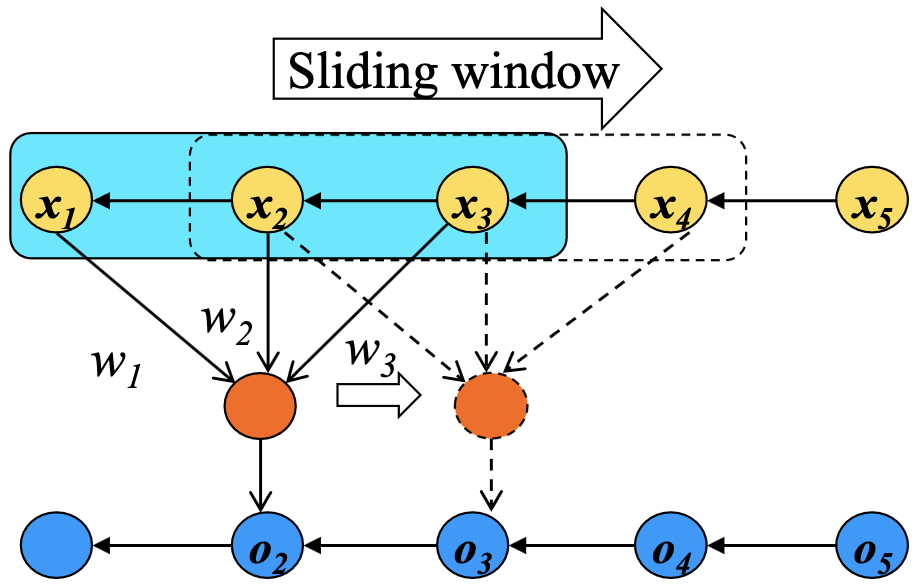
\includegraphics[width=0.45\linewidth]{img/CNN_simple.png}
\end{figure}

Here, the output of each node in the hidden layer is calculated as $out_t = \sum_{i=1}^3 w_i x_{t+i-2}$. In other words, the weights assigned to the inputs ``slide'' across the hidden layer. Weights are tuned as usual by learning.

\subsection{2D Convolution}

Discrete convolution can be seen as a multiplication by a matrix, with several entries constrained to be equal to other entries. The convolution over a 2D image $I$ with a kernel $K$ can be expressed as:
\begin{equation*}
    S(i,j) = (I*K)(i,j) = \sum_m \sum_n I(m,n)K(i-m, j-n) \,,
\end{equation*}
or, as expressed by many libraries, as the \textbf{cross-correlation function}:
\begin{equation*}
    S(i,j) = (I*K)(i,j) = \sum_m \sum_n I(i+m,j+n)K(i, j) \,.
\end{equation*}

The example below shows a 2D image with 25 pixels, and a 3x3 kernel (unit local receptive field) with a stride equal to 1 (i.e., the kernel moves across the image 1 pixel at a time; by choosing the stride we choose the size of the feature map). The image also has padding added to its edge.
\begin{figure}[h]
    \centering
    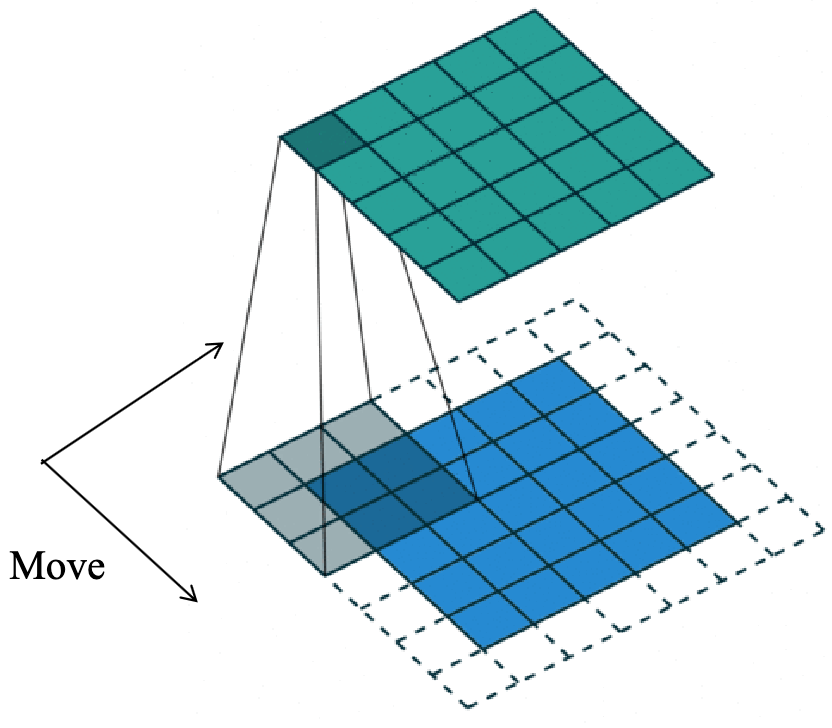
\includegraphics[width=0.6\linewidth]{img/CNN_2D.png} 
\end{figure}

Once the kernel reaches the end of the first ``row'' of pixels, it restarts from the position it started from shifted one pixel below. The full movement of the kernel over the image produces the feature map.

The image below better shows the matrix multiplication interpretation of convolution; the image is 4x3 and the kernel is 2x2. The stride is again equal to 1.

\begin{figure}[h]
    \centering
    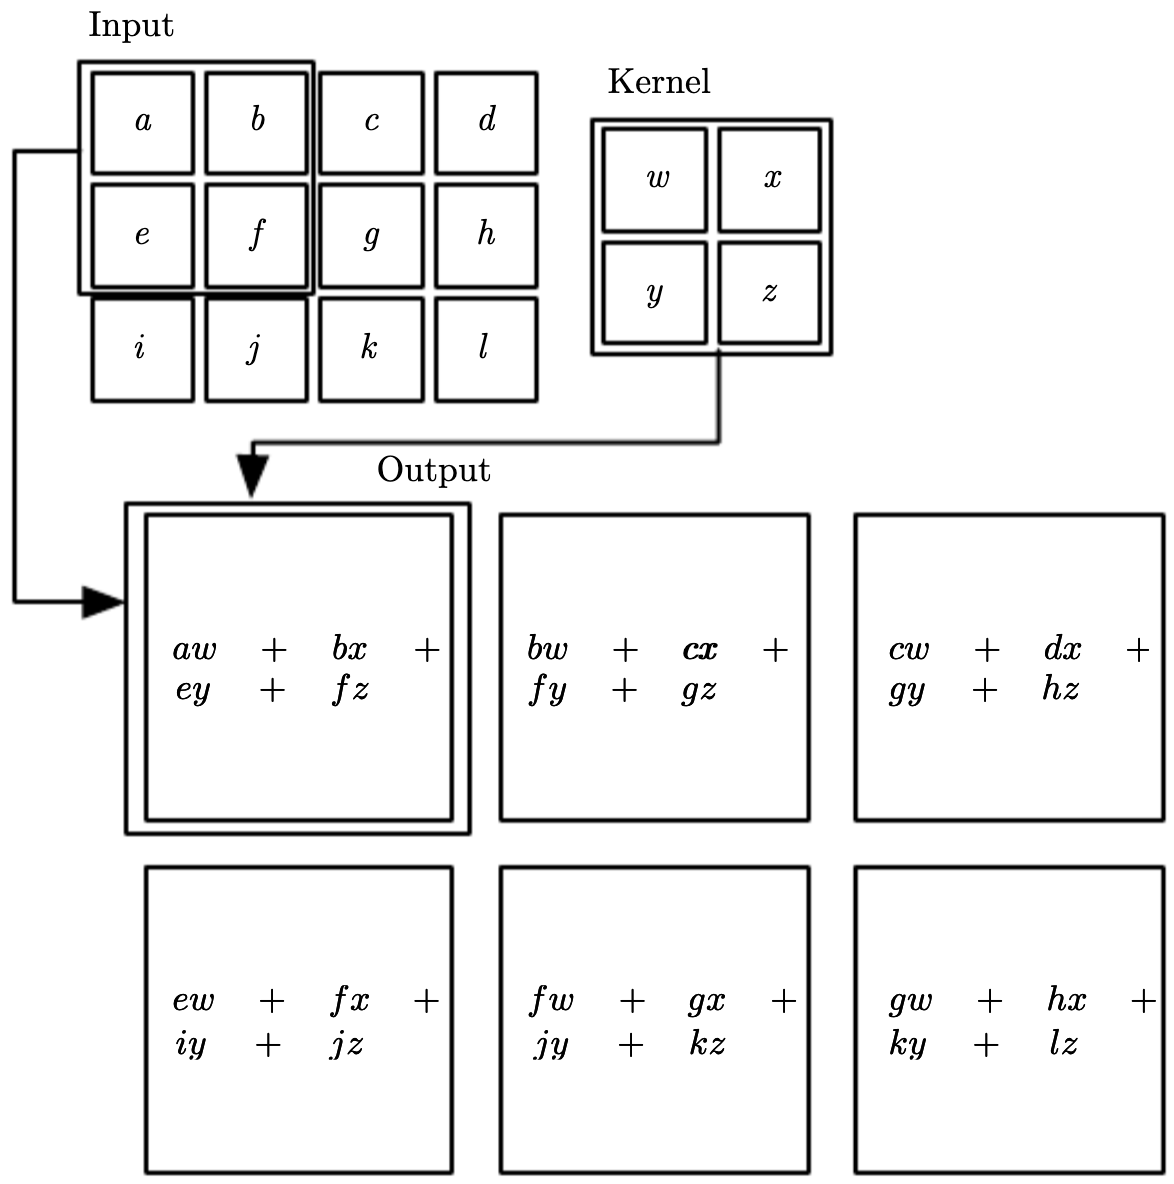
\includegraphics[width=0.5\linewidth]{img/CNN_matrix.png}
\end{figure}
Each unit's weights are a \textbf{filter} trained to detect some specific feature or pattern in the image. Each filter produces the strongest response to a spatially local input pattern, and then the filters obtained by training are applied to the whole (global) image, so that features and patterns can be identified regardless of where they are positioned on the image.

The size of the feature map can be reduced via pooling. Some examples of pooling are:
\begin{itemize}
    \item Subsampling, using a stride greater than 1;
    \item Calculating a mean (average or weighted average);
    \item Using the max pool operation (most common option).
\end{itemize}
This way, instead of producing a value for every single pixel of the original image, we get a smaller set of pixels where each value is obtained by considering the values of neighboring ones (calculating the mean or max value). Pooling also helps to make the representation approximately invariant to small translations of the input, since the mean or max value of a neighborhood of points is unlikely to be affected by a small translation of the pixels in the image.

CNN exploits \textbf{weight sharing}, where the number of connections in the network is kept the same while reducing the number of actual free parameters. The produced sliding window of units is applied over a segment of the input, and reapplied multiple times to produce various layers of feature maps. Training of the weights is usually done via backpropagation. Since these networks tend to be big and deal with large amount of data, many hyperparameters are fixed by experience or by suggestions of experts, since it would be too expensive to run cross-validation.

\section{Deep Learning}

The Deep Learning framework includes many different models, such as:
\begin{itemize}
    \item Deep Neural Networks;
    \item Convolutional Neural Networks;
    \item Deep belief Networks;
    \item Recurrent and Recursive Neural Networks.
\end{itemize}
They differ from ``shallow'' models in that they have a big amount of layers.

There's many different approaches to build a deep learning model. All these approaches have some aspects in common:
\begin{itemize}
    \item Multiple layers of nonlinear processing units;
    \item Supervised or unsupervised learning of feature representation in each layer, with the layers forming some hierarchy from low to high level features;
    \item Hierarchical sparse/distributed representation of the input data.
\end{itemize}

The core concept at the base of deep learning is increasing the level of abstraction of the data through the use of several layers; for example, an image can be gradually abstracted on each layer, first as a vector of intensity values per pixel, then a set of edges, then regions of a particular shape, and so on. We've already mentioned this idea with CNNs: the original complicated mapping is broken down into its simple elements, by gradually calculating simpler mapping at each layer. A series of hidden layers extracts increasingly abstract features from a set of example images. Additionally, these abstract features, once learned by the units, can also be combined together to generalize on examples that were never seen during training.

In general, deeper networks are often able to use less units per layer, thus less free parameters as well and less training data required to achieve a good generalization. Still, many layers may be harder to be trained, so there's a need to improve the techniques we know regarding gradient descent, regularization, and data exploitation.

\subsection{Insights}

\subsubsection{Why So Many Layers?}

Imagine a two-layer circuit of logic gates, which can represent any Boolean function. Any Boolean function can indeed be written as a sum of products (i.e., in disjunctive normal form). With logical circuits of depth two, the number of logic gates required to represent most Boolean functions is exponential w.r.t. input size.

An example of such function is the parity function: it returns 1 if there is an odd number of 1s over $N$ binary inputs (i.e., $N$ bits), 0 otherwise. If we were to implement this function with logic gates, assuming $N$ inputs, we would need:
\begin{equation*}
    \dfrac{2^N}{2} + 1 = 2^{N-1} + 1
\end{equation*}
gates, since we have to perform 1 OR and exactly $2^{N-1}$ ANDs.

We can propose an alternative solution with a polynomial number of gates, by increasing the number of layers to $log(N)$. The solution for $N=8$ is shown below (in a simplified view where each XOR corresponds to 3 AND gates and 1 OR gate). In this solution, the number of gates is greatly reduced from $2^7 + 1 = 129$ to only $7 * 3 = 21$.
\begin{figure}[h]
    \centering
    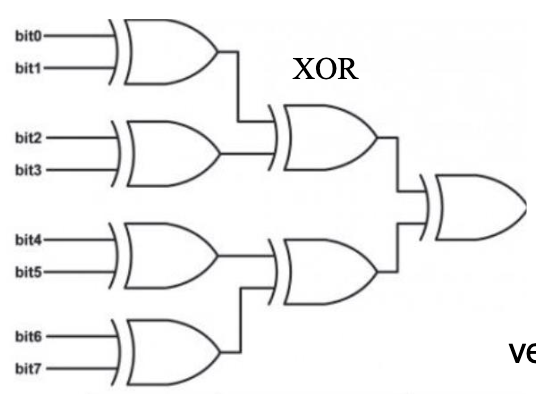
\includegraphics[width=0.5\linewidth]{img/Circuit_deep.png}
\end{figure}

The universal approximation theorem states that even with 1 hidden layer, a NN can approximate any possible function, however it does not specify the number of units needed. For some families of functions a boundary on this number can be found, but as seen in the example above, the bound may be exponential w.r.t. the dimension of the input. Also, there exist families of functions which can be approximated efficiently by a NN with depth greater than some value $d$, but which require a much larger model if depth is restricted to be less or equal than $d$.

This theorem also implies that regardless of what function we are trying to learn, a large MLP is able to represent the function, but there's no guarantee that that the training algorithm will be able to learn that function, either because it can't find the value of the parameters that correspond to the desired function, or because it might choose the wrong function due to overfitting. So another advantage to using multiple layers is ensuring that the learning algorithm can actually properly learn.

The inductive bias is: choosing a deep model encodes the (very general) belief that the function we want to learn should involve composition of several simple functions. If our task actually matches our bias, then the deep shape of the learner is suitable, and those deeper models also perform better than shallow ones. Typically, these tasks are the ones that involve images or language, but for other tasks that deal with different data this deep structure may not be appropriate.

Other challenges that motivate the usage of deep neural networks are related to the curse of dimensionality and manifold learning.

Recall that the curse of dimensionality is the phenomenon in which as the number of dimensions in the data increases, the less dense it is, thus becoming a problem for distance based machine learning algorithms. One challenge posed by this phenomenon is a statistical one: this challenge arises when the number of possible configurations of an input $x$ is much larger than the number of actual training examples. Let's say we want to estimate the probability density for some point $x$ by returning the number of training examples in the same unit volume cell as $x$ divided by the size of the training set. But if we want to estimate this density for a point that has no close neighbors within the unit volume cell (as is often the case when the dimensionality of data is high), there's no immediate way to calculate it. Additionally, even if present, neighbors are likely going to be very few. But deep learning is the solution: it can learn the single features it identifies in the training data, and those features can then be combined to produce an output even for instances that were never seen before.

A manifold is a connected region. Mathematically, it's a set of points associated with a neighborhood around each point. From any given point, the manifold locally appears to be a Euclidean space. As an example, in the real world, we experience the surface of the Earth as 2D, but in reality it's a sphere in 3D space. In the case of Machine Learning, ``manifold'' is a term used to broadly refer to a connected set of points that can be approximated well by considering only a small number of dimensions. Different points can also have a different number of dimensions, typically when the manifold intersects itself. \textbf{Manifold learning} assumes that the only interesting inputs occur only along a collection of manifolds containing a small subset of points, with interesting variations in the output occurring only across directions that lie on the manifold, or only when moving from one manifold to the other. This assumption is often used for data types such as images, text, or audio that occur in real life, since uniform, artificial noise never resembles the inputs from those domains, so the probability distribution of the only valid data is highly concentrated. *?

\subsection{Representation Learning}

With Deep Learning, other concepts are emerging, such as representation learning, which is the set of methods that automatically discover the best representation of raw data for some other task. It's especially useful for more complex data types like images, text, or audio data. Deep Learning methods are also representation learning methods with multiple levels of representation.

The reason behind representation learning is that many information processing tasks can have varying difficulty based on the way the information is represented. In Machine Learning, a good representation is one that makes a subsequent learning task easier. Supervised learning in MLPs is an example that leads to an automatic representation at every hidden layer taking on properties that make the output layer task easier (think of the XOR example). Another example is CNNs, since they take as input a raw image and automatically learn to identify the main features of the image, decomposing it into its parts.

The hidden representation of data can be obtained via \textbf{pretraining approaches}, semi-supervised learning, which means we can learn a representation for the unlabeled data and use it to solve supervised tasks. The representation can be then exploited with \textbf{transfer learning} approaches.

\textbf{Greedy Layer-Wise Unsupervised Pretraining} was the first approach to make it possible to train a deep supervised network. It makes the training of the whole network much easier, since there's no need for an end-to-end training from the output layer to the previous hidden layers with a gradient descent, which used to be difficult for deep models. The adjective ``greedy'' refers to the fact that each layer is optimized independently in an unsupervised way. This methods works not only as a good initialization strategy, but also as regularization regarding the complexity of the original data, since it extracts the features that simplify the unsupervised process. It also reduces the variance of the estimation training process, since pretrained models tend to gather in a smaller region after training).

Before continuing, let's explain what are \textbf{autoencoders}. An autoencoder is a neural network that is trained to attempt to copy its input to its output. It has a hidden layer $h$ that describes a \textbf{code} used to represent the input. The network can be seen as two components: the encoder function $h = f(x)$, and the decoder $r = g(h)$ that produces a reconstruction. Autoencoders are specifically trained so that they are unable to copy the input perfectly, but instead only copy parts of the data or copy it only approximately.